\documentclass[]{article}
\usepackage{amsmath}
\usepackage{graphicx}
\usepackage{caption}
\graphicspath{{C:\Users\Vale\Dropbox\Poli\Erasmus\KTH\Statitical Methods for Applied Computer Science\DD2447_2017}}

% Title Page
\title{Statistical Methods in \\ Applied Computer Science, Fall 2017 \\ Assignment 2}
\author{Valeria Callioni, Viran Ribi\'c , \\ Assignment 2 Group 3}


\begin{document}
\maketitle

\newpage

\section*{2.1 SMC for the stochastic volatility model}
In this first task we have to consider the stochastic volatility model
\begin{align*}
	X_t|X_{t-1} = x_{t-1} \sim \mathcal{N}(x_t | \phi x_{t-1},\sigma^2), && t=1...T 
	\\
	Y_t|X_t = x_t \sim \mathcal{N}(y_t | 0, \beta^2e^{x_t}), && t=1...T 
\end{align*}
where we assume stationarity by setting 
$$
X_0 \sim \mathcal{N}(x_0 | 0, \frac{\sigma^2}{1-\phi^2})
$$
The latent variable $X_t$ denotes the underlying volatility, i.e. the variations in the price of some financial asset, and $Y_t$ denotes the observed scaled log-returns from the asset. 
First we generate parameters together with a synthetic data vector $y_{1:T}$, $T = 500$, based on the stochastic volatility model, using the generator provided; then we implement a SMC algorithm with and without resampling with the final goal of estimating the likelihood for different values of the parameter $\beta$, considering the other parameters to be known. 

Let us explain the setting. We analyzed it using the paper "A Tutorial on Particle Filtering and Smoothing: Fifteen years later", as theoretical support. $\{X_t\}_{t\geq0}$ is a discrete-time Markov process such that 
$$
X_0 \sim \mu(x_0) \text{ and } X_t|X_{t-1} = x_{t-1} \sim f(x_t|x_{t-1})
$$
We are interested in estimating $\{X_t\}_{t\geq0}$ but only have access to the values of the process $\{Y_t\}_{t\geq1}$. We assume that, given $\{X_t\}_{t\geq0}$, the observations $\{Y_t\}_{t\geq1}$ are statistically independent and their marginal densities are given by
$$
Y_t|X_t = x_t \sim g(y_t|x_t).
$$
We also assume that the transition and observation densities are independent of the time index $n$. This leads to a Bayesian model with the prior distribution given by 
$$
p(x_{0:T}) = \mu(x_0)\prod_{t=1}^{T}f(x_t|x_{t-1})
$$
and the likelihood
$$
p(y_{1:T}|x_{0:T}) = \prod_{t=1}^{T}g(y_t|x_t).
$$
Then the posterior distribution is
$$
p(x_{0:T}|y_{1:T}) = \frac{p(x_{0:T},y_{1:T})}{p(y_{1:T})}.
$$
Since our final goal is to determine the log-likelihood of the data for different values of the parameter $\beta$, we want to approximate $p(y_1)$ at the first time instance, $p(y_{1:2})$ at the second time instance and so on.

We want to use SMC methods, a general class of Monte Carlo methods that sample senquentially from a sequence of target probability densities $\{ \pi_t(x_{1:t}) \}$ of increasing dimension. In particular, 
$$
\pi_t(x_{0:t}) = \frac{\gamma_t(x_{0:t})}{Z_t}
$$
where 
$\gamma_t$ is known pointwise and the normalizing constant $Z_t$ is known.

In our particular case, that can be consideres as a Filtering problem, we have
$$
\gamma_t(x_{1:t}) = p(x_{0:T},y_{1:T})
$$ 
that means
$$
\pi_t(x_{0:t}) = p(x_{0:T}|y_{1:T}) \text{ and } Z_t = p(y_{1:t}).
$$
Then, the proposal distibution is given by 
$$
q_t(x_t|x_{0:t-1}) = q_t(x_t|y_t, x_{t-1})
$$
that leads to incremental weights of the form
$$
\alpha_t(x_{0:t}) = \alpha_t(x_{t-1:t}) = \frac{g(y_t|x_t)f(x_t|x_{t-1})}{q_t(x_t|y_t, x_{t-1})}.  
$$
In our setting, the conditional prior can be employed as a proposal distribution. Then, the incremental weights are simply given by
$$
\alpha_t(X_{t-1:t}^i) = g(y_t|X_t^i).
$$
To obtain the log-likelihood, at each iteration we have to compute
\begin{align*}
	\log\hat{p}(y_{1:t}) = & \log[ \hat{p}(y_1) \prod_{k=2}^{t} p(y_k|y_{1:k-1})] \\
	= & \log \hat{p}(y_1) + \sum_{k=2}^{t} \log p(y_k|y_{1:k-1})
\end{align*}
where
\begin{align*}
	\hat{p}(y_1) = & \sum_{i=1}^{N} p(y_1|X_1^i)p(X_1^i) \\
	= & \sum_{i=1}^{N} p(y_1|X_1^i)[\sum_{j=1}^{N}p(X_1^i|X_0^j)p(X_0^j)] \\
	= & \sum_{i=1}^{N} g(y_1|X_1^i)[\sum_{j=1}^{N}f(X_1^i|X_0^j)\mu(X_0^j)]
\end{align*}
and
$$
\hat{p}(y_t|y_{1:t-1}) = \sum_{i=1}^{N}W_{n-1}^i\alpha_t(X_{t-1:t}^i).
$$
\subsection*{Question 1}
Following this reasoning, we implemented the SMC algorithm. The first step is given by the initialization, that is 
\begin{enumerate}
	\item[-] sample $X_0^i \sim \mathcal{N}(0, \frac{\sigma^2}{1-\phi^2})$
	\item[-] sample $X_1^i \sim \mathcal{N}(\phi x_0^i,\sigma^2) $ 
	\item[-] compute the weights $w_1(X_1^i) = \sum_{j=1}^{N}f(X_1^i|X_0^j)\mu(X_0^j)$ and the normalized weights $W_1(X_1^i)$
	\item[-] compute the incremental weights $ \alpha_1(X_1^i) = g(y_1|X_1^i)w_1(X_1^i) $
	\item[-] compute $\log \hat{p}(y_1)$ as previously stated. 
\end{enumerate}
Then, at each iteration $t \geq 2$:
\begin{enumerate}
	\item[-] sample $X_t^i \sim \mathcal{N}(\phi x_{t-1}^i,\sigma^2) $
	\item[-] compute the incremental weights $ \alpha_t(X_{t-1:t}^i) = g(y_t|X_t^i) $
	\item[-] compute $\log \hat{p}(y_t|y_{1:t-1})=\log\sum_{i=1}^{N}W_{t-1}^i\alpha_t(X_{t-1:t}^i)$
	\item[-] compute the weights $
	w_t(X_{0:t}^i)=w_0(X_1^i)\prod_{k=2}^{t}\alpha_k(X_{0:k}^i)$ and the normalized weights
\end{enumerate}
Considering a coarse grid for $\beta$, given by 20 points equally-spaced in the interval $(0,2)$ and running 10 times the SMC for every value of $\beta$, we obtained the result presented in Figure 1. 
\begin{figure}
	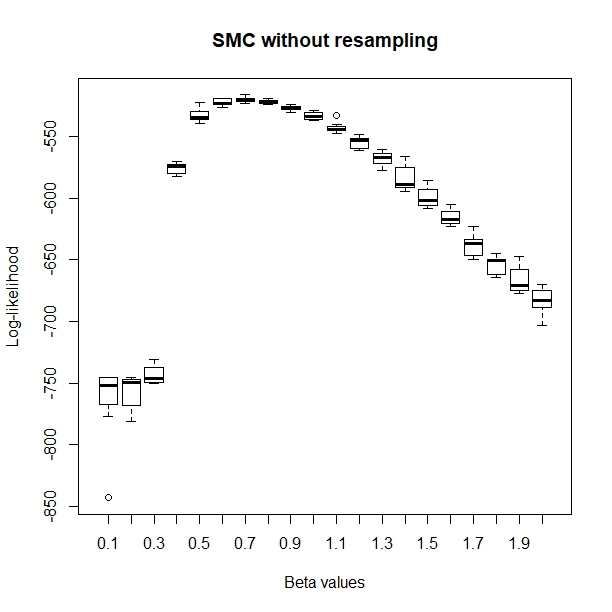
\includegraphics[width=\columnwidth]{task1/SIS_N_10000_T_500.jpeg}
	\caption{Log-likelihood running SIS 10 times, with $N=10^4$ and $T=500$}
\end{figure}
The data were generated with the following parameters values: $\phi = 0.97$, $\sigma=0.13$ and $\beta=0.67$. From Figure 1 we can see that the maximum value of the log-likelihood is reached, in mean, for $\beta=0.7$.

\subsection*{Question 2}
Introducing resampling means to sample from an approximation $\hat{\pi}(x_{1:t})$ which was itself obtained by sampling. We resample $N$ times from $\hat{\pi}(x_{1:t})$, which is equivalent to associating a number of offspring $N_t^i$ with each particle $X_{1:t}^i$ in such a way that $N_t^{1:N} = (N_t^1, ..., N_t^N)$ follow a multinomial distribution with parameter vector $(N, W_t^{1:N})$ and associating a weight of $\frac{1}{N}$ with each offspring. Since we use systematic resampling, the previous algorithm becomes as follows:

Initialization:
\begin{enumerate}
	\item[-] sample $X_0^i \sim \mathcal{N}(0, \frac{\sigma^2}{1-\phi^2})$
	\item[-] sample $X_1^i \sim \mathcal{N}(\phi x_0^i,\sigma^2) $ 
	\item[-] compute the weights $w_1(X_1^i) = \sum_{j=1}^{N}f(X_1^i|X_0^j)\mu(X_0^j)$ and the normalized weights $W_1(X_1^i)$
	\item[-] compute the incremental weights $ \alpha_1(X_1^i) = g(y_1|X_1^i)w_1(X_1^i) $
	\item[-] sample $U_1 \sim \mathcal{U}[0, \frac{1}{N}]$ and define $U_i = U_1 + \frac{i-1}{N}$
	\item[-] set $N_1^i = |\{ U_j: \sum_{k=1}^{i-1}W_1^k \leq U_j \leq \sum_{k=1}^{i}W_1^k \}|$ with the convention $\sum_{k=1}^{0}=0$, and set the particles to be $N$ equally-weighted of the form $\{\frac{1}{N}, X_1^i\}$
	\item[-] update the values of the incremental weights  $ \alpha_1(X_1^i) $ given the new equally-weighted particles
	\item[-] compute $\log \hat{p}(y_1)$. 
\end{enumerate}
Then, at each iteration $t \geq 2$:
\begin{enumerate}
	\item[-] sample $X_t^i \sim \mathcal{N}(\phi x_{t-1}^i,\sigma^2) $
	\item[-] compute the incremental weights $ \alpha_t(X_{t-1:t}^i) = g(y_t|X_t^i) $
	\item[-] sample $U_1 \sim \mathcal{U}[0, \frac{1}{N}]$ and define $U_i = U_1 + \frac{i-1}{N}$
	\item[-] set $N_t^i = |\{ U_j: \sum_{k=1}^{i-1}W_t^k \leq U_j \leq \sum_{k=1}^{i}W_t^k \}|$ with the convention $\sum_{k=1}^{0}=0$, and set the particles to be $N$ equally-weighted of the form $\{\frac{1}{N}, X_t^i\}$
	\item[-] update the values of the incremental weights  $ \alpha_t(X_{t-1:t}^i) $ given the new equally-weighted particles
	\item[-] compute $\log \hat{p}(y_t|y_{1:t-1})=\log\sum_{i=1}^{N}\frac{1}{N}\alpha_t(X_{t-1:t}^i)$
	\item[-] compute the weights $
	w_t(X_{0:t}^i)=w_0(X_1^i)\prod_{k=2}^{t}\alpha_k(X_{0:k}^i)$ and the normalized weights
\end{enumerate}
Considering the same coarse grid for $\beta$, the same data as before, and running 10 times the SMC with resampling for every value of $\beta$, we obtained the result represented in the follwing figure. We ran the SIR algorithm 10 times,  with $N=10^3$ and $T=500$.
\\
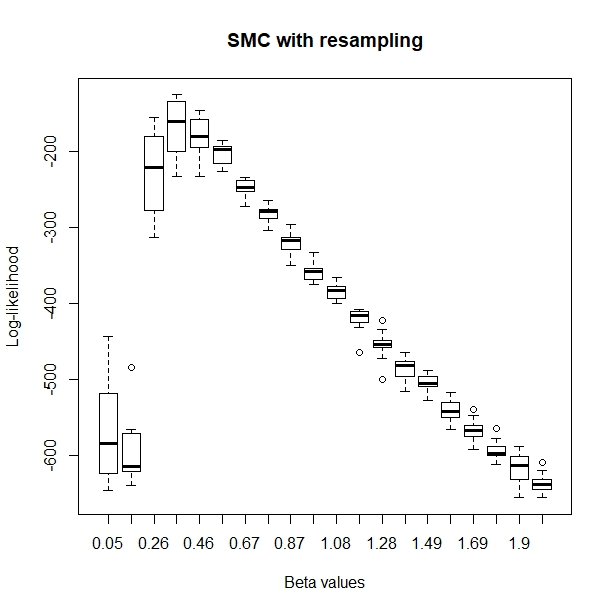
\includegraphics[width=\columnwidth]{task1/SIR_N_1000_T_500.jpeg}

\subsection*{Question 4}
Finally, we run the algorithm with different values of $T$ and $N$, to study how these parameters affect the variance in the log-likelihood estimate. 

\begin{figure}
	\begin{center}
		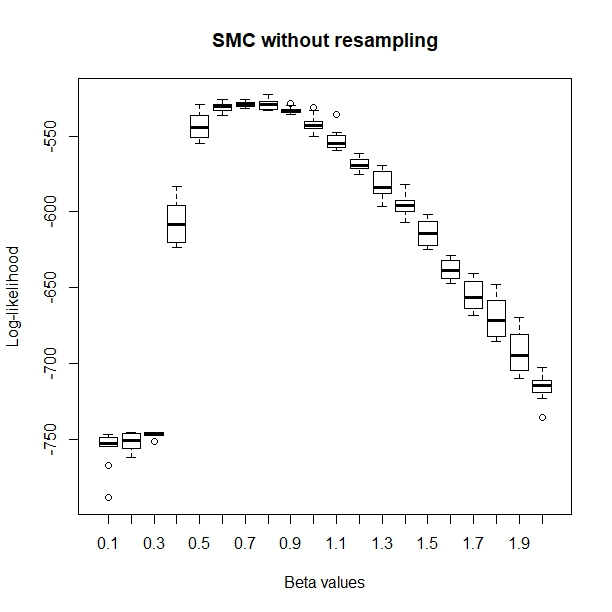
\includegraphics[width=.4\textwidth]{task1/SIS_N_1000_T_500.jpeg}
		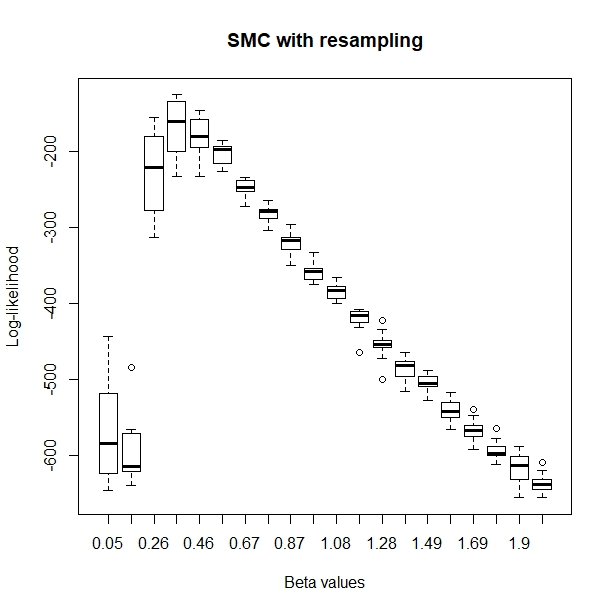
\includegraphics[width=.4\textwidth]{task1/SIR_N_1000_T_500.jpeg}
		\caption*{$N=10^3$ and $T=500$}
		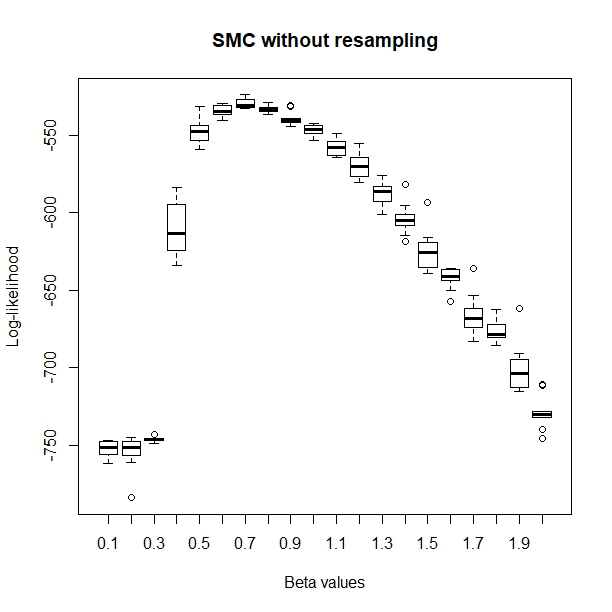
\includegraphics[width=.4\textwidth]{task1/SIS_N_500_T_500.jpeg}
		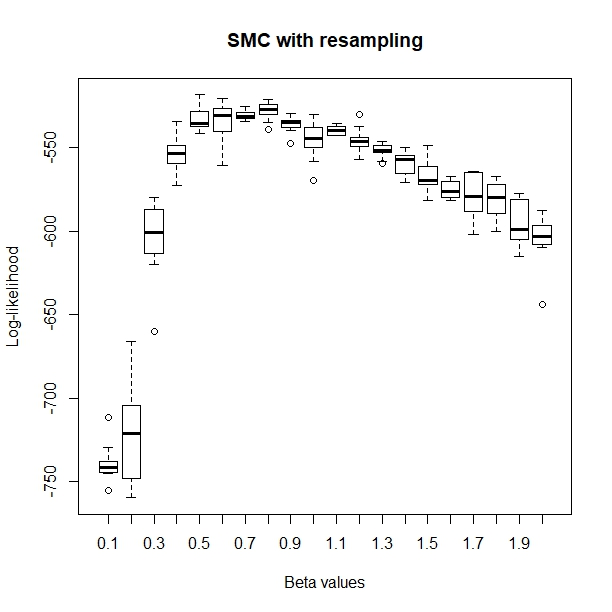
\includegraphics[width=.4\textwidth]{task1/SIR_N_500_T_500.jpeg}
		\caption*{$N=500$ and $T=500$}
		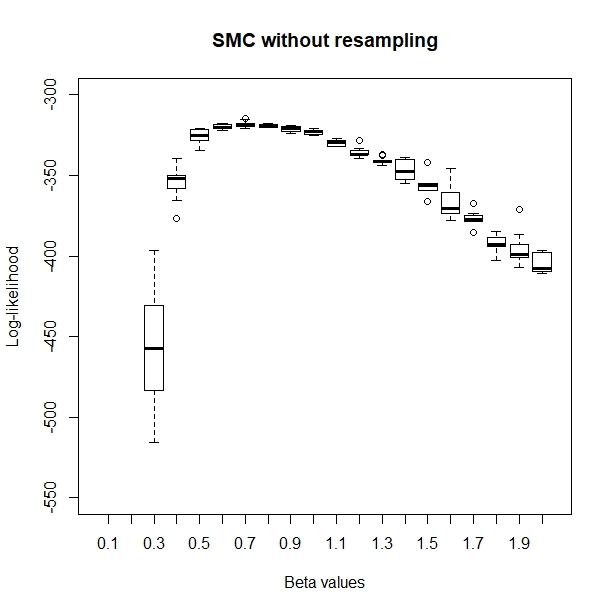
\includegraphics[width=.4\textwidth]{task1/SIS_N_1000_T_300.jpeg}
		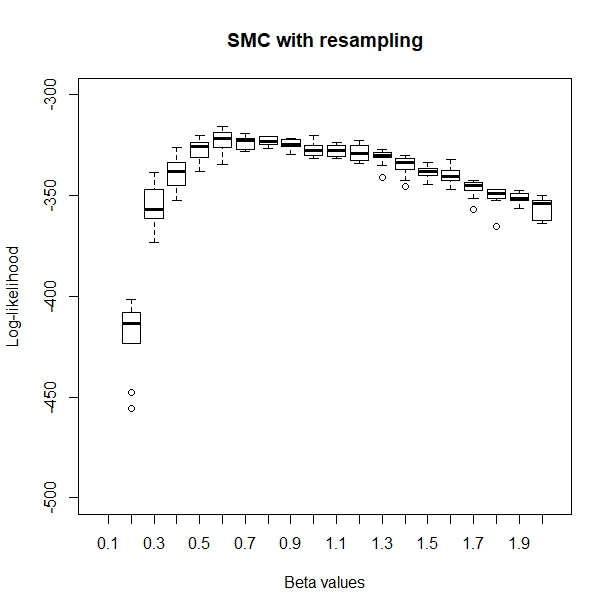
\includegraphics[width=.4\textwidth]{task1/SIR_N_1000_T_300.jpeg}
		\caption*{$N=10^3$ and $T=300$}
	\end{center}
	\caption{Comparison of the results for different values of $T$ and $N$}
\end{figure}

From Figure 3, we observe that for smaller values of T we have a smaller variance in the estimator, especially in the SMC without resampling. This is due to the fact that for large values of $T$ the particle filtering may degenerate. But, in any case, the SIR algorithm performs better than the SIS one, as we expect. 

\newpage

\section*{2.3 MCMC for the train}
We are given a problem that models a railway with a single train. The map of the tracks is represented by an undirected graph $G=(V,E)$, such that each node has degree 3 and at each vertex edges are labeled $0, L or R$. Each vertex represents a switch: if the train comes from the direction of $L$ or $R$, it always leaves in the direction 0; if the train comes from the direction $0$, it will leave in either direction $L$ or $R$, depending on the state of the switch. The switch has prior probability 1/2 for each direction, but will remain the same throughout the train run. A switch setting is a function $\alpha : V(G) \rightarrow \{L,R\}$

We observe a sequence of $T$ signals, each one representing the label of the edge through which the train has exited a vertex. But the sensors are noisy, and with probability $p = 0.05$, the train reports a random other signal than real direction in which it passed the switch. 

We are given a DP algorithm to compute $p(s,O|G,\alpha)$, where $s=(v,e)$ is called stop position; and the final goal is to estimate the probability distribution of the vector $\alpha(\mathbf{v}) = (\alpha(v_1), ..., \alpha(v_N))$,  where $ N=|V(G)| $, using MCMC.

\subsection*{Question 8}
We implemented the class $Graph$ to generate the map of the railway. This class has the following attributes:
\begin{enumerate}
	\item[-] $V$, the number of nodes 
	\item[-] the degree of the graph ($degree=3$ in our setting) 
	\item[-] $A$, the adjacency matrix, where $A_{ij}=1$ if edge $(i,j)$ exists and $A_{ij}=0$ otherwise
	\item[-] $G$, the matrix representing the labels of the edges, where $G_{ij} \ \in \ \{ 0,1,2,3\} $. We used the convention that 0 represents 0, 1 represents $L$, 2 represents $R$ and 3 is assigned to edges that do not exist.
\end{enumerate} 
The map is created randomly, being sure that each vertex has degree 3 and assigning the 3 different labels to the existing edges.

The class $Train$ actually represents our setting: it has a graph, the map; the vector of obervations $O$ and the associated $path$. Observations are generated randomly and, in the end, some noise is added.

In the MCMC Metropolis Hastings algorithm that we propose, states are switch settings vectors and, at each step, the algorithm performs the following operations:
\begin{enumerate}
	\item[-] propose a new switch setting vector, by simply picking a random vertex and changing its setting. The candidate new state is chosen in this way since we have no particular assumptions and we decided to consider a uniform proposal distribution;
	\item[-] accept the new switch setting with acceptance probability 
	$$
	r(\mathbf{\alpha}_{new}|\mathbf{\alpha}_{old}) = min\{1, a(\mathbf{\alpha}_{new}|\mathbf{\alpha}_{old})\},
	$$
	where
	$$
	a(\mathbf{\alpha}_{new}|\mathbf{\alpha}_{old}) = \frac{p^*(\mathbf{\alpha}_{new})}{p^*(\mathbf{\alpha}_{old})}\frac{q(\mathbf{\alpha}_{old}|\mathbf{\alpha}_{new})}{q(\mathbf{\alpha}_{new}|\mathbf{\alpha}_{old})} 
	$$
	where $p^*$ is the target distribution and $q$ is the proposal distribution, which we assume to be symmetric. So,
	$$
	a(\mathbf{\alpha}_{new}|\mathbf{\alpha}_{old}) = \frac{p(D|\mathbf{\alpha}_{new})}{p(D|\mathbf{\alpha}_{old})} \frac{p(\mathbf{\alpha}_{new})}{p(\mathbf{\alpha}_{old})}
	$$
	Since we have uniform prior for the switch setting of each node and we assume switch settings of different nodes to be independent, and since our data $D$ are given by the vector of observations $\mathbf{O}$ we have
	$$
	a(\mathbf{\alpha}_{new}|\mathbf{\alpha}_{old}) = \frac{p(\mathbf{O}|G,\mathbf{\alpha}_{new})}{p(\mathbf{O}|G,\mathbf{\alpha}_{old})}
	$$
	The probability $p(\mathbf{O}|G,\mathbf{\alpha})$ can be computed using the DP algorithm provided, since it suffices to sum over the all possible stop positions, given particular switch settings. 
\end{enumerate}
At the end we obtain sample switch settings, that we store just after the $burn-in$ phase, and their associated probability.

\subsection*{Question 9}
To run the program, we set $V=6$ and $O=6$. We decided not to consider too many nodes, since otherwise the probabilities associated to the switch setting vectors would have been very small. Setting $V=6$ we expect to understand the results of the MCMC algorithm. Furthermore, first we considered $N=10^3$, that leads to have $10^3$ samples that will actually be considered in the results, and $500$ initial iterations that will be considered as belonging to the \emph{burn-in} phase. The result that we obtained is the following:
\begin{center}
	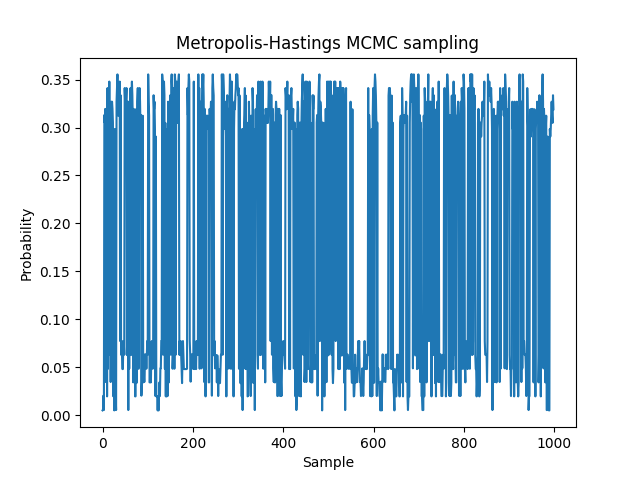
\includegraphics[height=7cm]{task3/V_6_T_6_N_1000.png}
\end{center}
We can observe that the probability distribution provided by the sampling is quite stable.

To understand the accuracy of the method, we compared the true switch settings with the most likely, according to the result. The most likely switch settings are the ones that were chosen most often during the sampling. 
\begin{center}
	\begin{tabular}{| c | c | c | c | c | c | c |}
		True $\alpha(\mathbf{v})$ & $R$ & $L$ & $L$ & $R$ & $R$ & $L$ \\
		ML $\alpha(\mathbf{v})$ & $R$ & $L$ & $R$ & $R$ & $R$ & $L$ \\
	\end{tabular}
\end{center}
In particular, we provide the plot of the MCMC Metropolis Hastings label proposals for node 1.
\begin{center}
	\begin{tabular}{| c |}
		$p(\alpha(v_1)=L) = 0.46 $ \\
		$p(\alpha(v_1)=R) = 0.54 $ \\
	\end{tabular}
\end{center}
\begin{center}
	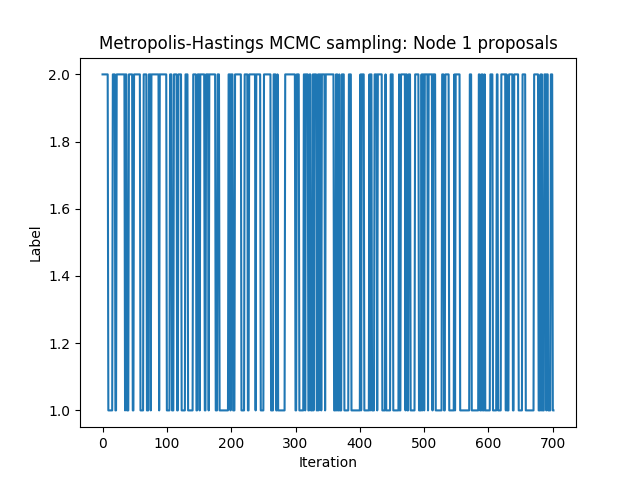
\includegraphics[height=6.8cm]{task3/V_6_T_6_N_1000_Node1.png}
\end{center}
Running again the program, performing $N=10^4$ iterations, we have the following results:
\begin{center}
	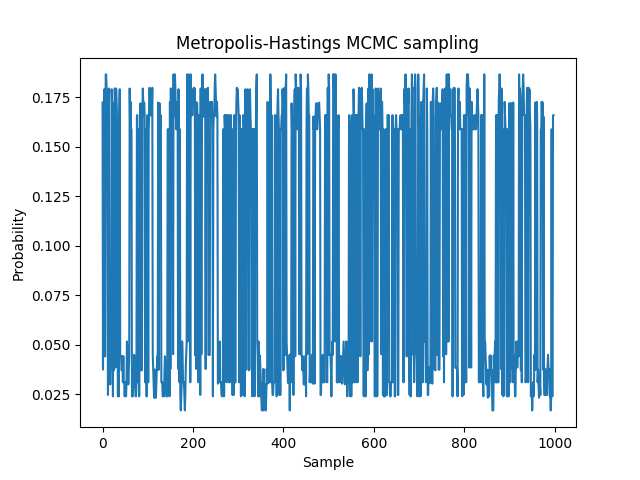
\includegraphics[height=7cm]{task3/V_6_T_6_N_10000.png}
	\begin{tabular}{| c | c | c | c | c | c | c |}
		True $\alpha(\mathbf{v})$ & $R$ & $R$ & $L$ & $L$ & $R$ & $R$ \\
		ML $\alpha(\mathbf{v})$ & $R$ & $R$ & $L$ & $R$ & $R$ & $L$ \\
	\end{tabular}
	\\
	\begin{tabular}{| c |}
		$p(\alpha(v_1)=L) = 0.51 $ \\
		$p(\alpha(v_1)=R) = 0.49 $ \\
	\end{tabular}
\end{center}
Note that in the plots we show just the last $10^3$ iterations to make them more clear to the reader. 

\subsection*{Question 10}
Now, we aim to perform the same analysis using Gibbs sampling instead of Metropolis Hastings. So, at each iteration $i = 1...N$
\begin{enumerate}
	\item[-] sample $\alpha(v_1)$, 
	\item[-] sample $\alpha(v_2)$,
	\item[-] ...
	\item[-] sample $\alpha(v_V)$,  
\end{enumerate} 
In particular, for each node $j \in V(G)$, the sampling step is done according to
$$
\text{with probability } \frac{1}{2} \text{, } \alpha(v_j^{i+1}) = \alpha(v_j^i)
$$
$$
\text{with probability } \frac{1}{2} \text{, } \alpha(v_j^{i+1}) \neq \alpha(v_j^i)
$$
Setting $V=6$, $T=6$ and $N=10^4$, we obtained
\begin{center}
	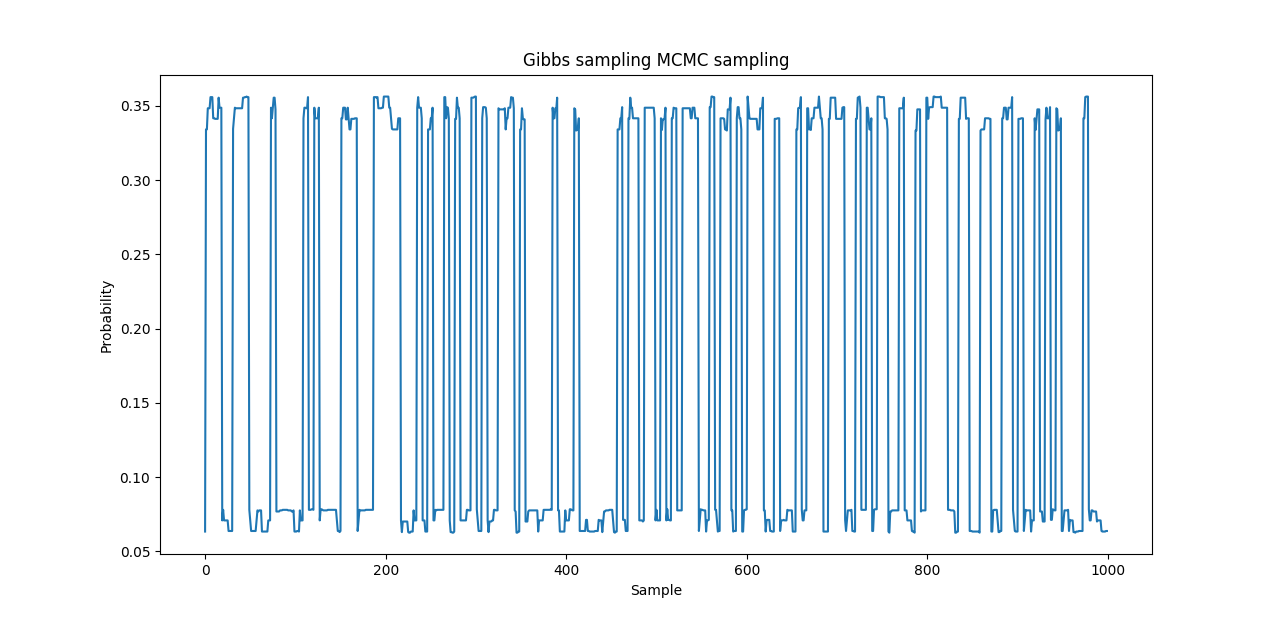
\includegraphics[width=\columnwidth]{task3/V_6_T_6_N_10000_Gibbs.png}
	\begin{tabular}{| c | c | c | c | c | c | c |}
		True $\alpha(\mathbf{v})$ & $R$ & $R$ & $L$ & $L$ & $R$ & $R$ \\
		ML $\alpha(\mathbf{v})$ & $R$ & $R$ & $R$ & $L$ & $L$ & $R$ \\
	\end{tabular}
\end{center}
Considering blocked Gibbs sampling, we can say that the Metropolis Hasting algorithm proposed in the previous part of the task corresponds to blocked Gibbs with blocked size equal to $V$, since in MH we change randomly one component of the switch setting vector at each iteration. We could consider any size for blocked Gibbs: if we consider $n \leq V$ ($n > 1$) groups of components at each iteration, then we change randomly $n$ switch settings of $\alpha(\mathbf{v})$.

For instance, we run the blocked Gibbs sampling for $n=2$ with $V=6$, that means that we consider at each iteration 3 groups of components. We obtained a more accurate result:
\begin{center}
	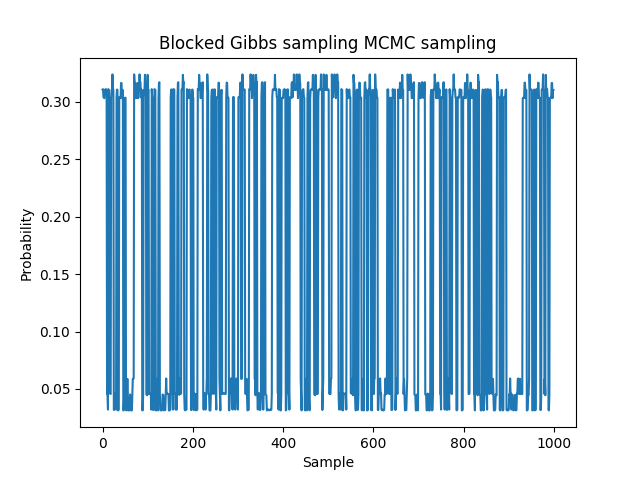
\includegraphics[height=6cm]{task3/V_6_T_6_N_10000_Blocked_Gibbs.png}
	\begin{tabular}{| c | c | c | c | c | c | c |}
		True $\alpha(\mathbf{v})$ & $L$ & $R$ & $L$ & $R$ & $R$ & $R$ \\
		ML $\alpha(\mathbf{v})$ & $L$ & $R$ & $L$ & $R$ & $R$ & $R$ \\
	\end{tabular}
\end{center}

In our sampling algorithms we do not need to sample the stop position $s$ for the reasoning about proposals and acceptance probabilities that we provided at the beginning of the task. However, we could compute the probability associated to each stop position given the switch settings. 

\newpage

\section*{2.5 Stochastic volatility unknown parameter}
Let us consider the problem presented in task 2.1. Now, we assume that the variance parameters $\sigma$ and $\beta$ are both unknown, while $\phi$ is given. The Bayesian setting is characterized by the priors:
$$
\sigma^2 \sim \mathcal{IG}(a=0.01, b=0.01)
$$
$$
\beta^2 \sim \mathcal{IG}(a=0.01, b=0.01)
$$
Then, we obtain the posterior distributions of the variance parameters in closed form:
$$
p(\sigma^2|\phi, x_{0:T}, y_{1:T}) = \mathcal{IG}(\sigma^2|a+\frac{T}{2}, b+\frac{1}{2}\sum_{t=1}^{T}(x_t-\phi x_{t-1})^2)
$$
$$
p(\beta^2|\phi, x_{0:T}, y_{1:T}) = \mathcal{IG}(\sigma^2|a+\frac{T}{2}, b+\frac{1}{2}\sum_{t=1}^{T}e^{-x_t}y_t^2)
$$

\subsection*{Question 13}
We implemented a particle Gibbs sampler to compute the posterior distribution $p(\sigma^2, \beta^2|\phi, y_{1:T})$. To do so, at each iteration we alternatively sample from
\begin{enumerate}
	\item[-] $p(\sigma^2|\phi, x_{0:T}, y_{1:t})$
	\item[-] $p(\beta^2|\phi, x_{0:T}, y_{1:t})$
	\item[-] $p(x_{0:T}|\theta, y_{1:T})$
\end{enumerate}
The initialization is perfomed considering as first value of $\sigma$ the true value, i.e., $\sigma = 0.1315$. In this problem, $\phi = 0.9709$. Then we sample the first values of $x_t$, for $t=0...T$, considering the distributions presented in task 2.1.

Considering $N=10^4$ and $T=500$, with a $burn-in$ fase of 5000 iterations, we obtained the following marginal distributions for the variance parameters:
\begin{center}
	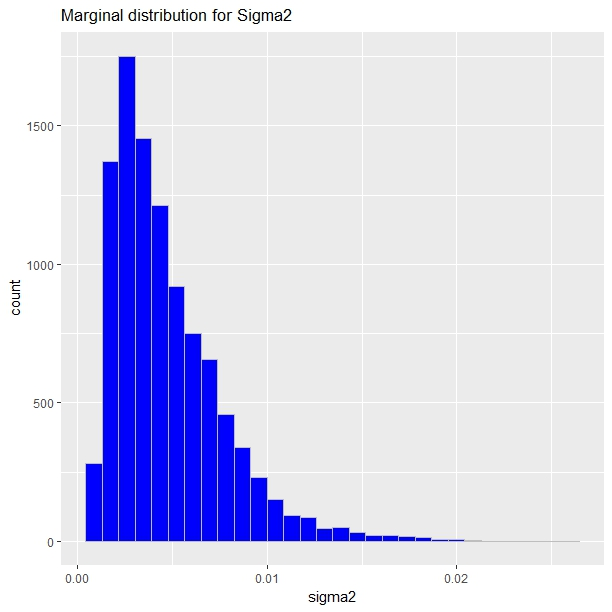
\includegraphics[width=.4\textwidth]{task5/Gibbs_sigma2.jpeg}
	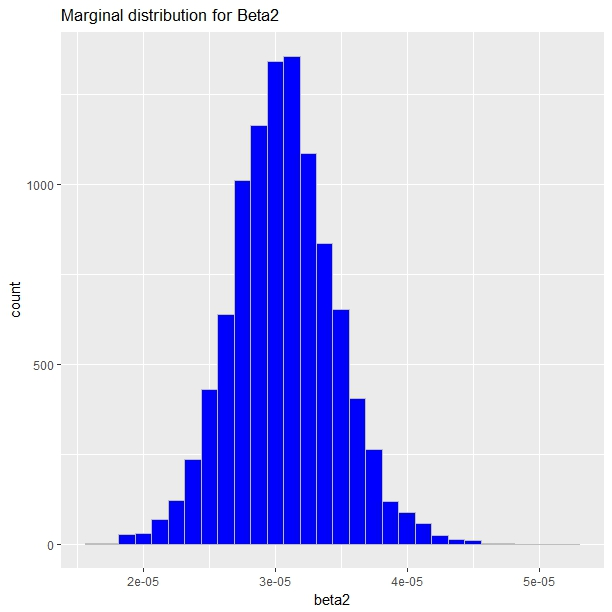
\includegraphics[width=.4\textwidth]{task5/Gibbs_beta2.jpeg}
\end{center}


\subsection*{Question 14}
We tried to implement a Particle MCMC sampler for this model, by reusing the SMC implemented in 2.1, now modifed to become a Conditional SMC. 

Our implementation works as follows: first we initialize $\sigma$ and $\beta$ to their correct values; then we initialize $x_{0:T}$ using the distributions given in task 2.1; we perform once the SMC (with resampling), and the output is a $(T+1) \times N$ matrix, that we need for the Conditional Sequential Monte Carlo.

The sampling part has the following steps:
\begin{enumerate}
	\item we sample $\sigma^2$ from $p(\sigma^2|\phi, x_{0:T}, y_{1:t})$;
	\item we sample $x_{0:T}$ running again the SMC algorithm, where  the $N^{th}$ particle's path is unchanged, with respect to the first SMC that we run. The sampling is performed by picking a random index $j$ in $\{1,...,N-1\}$ and considering the path of the $j^{th}$ particle;
	\item we sample $\beta^2$ from $p(\beta^2|\phi, x_{0:T}, y_{1:t})$.
\end{enumerate}

We obtained the following marginal distributions for the variance parameters:
\begin{center}
	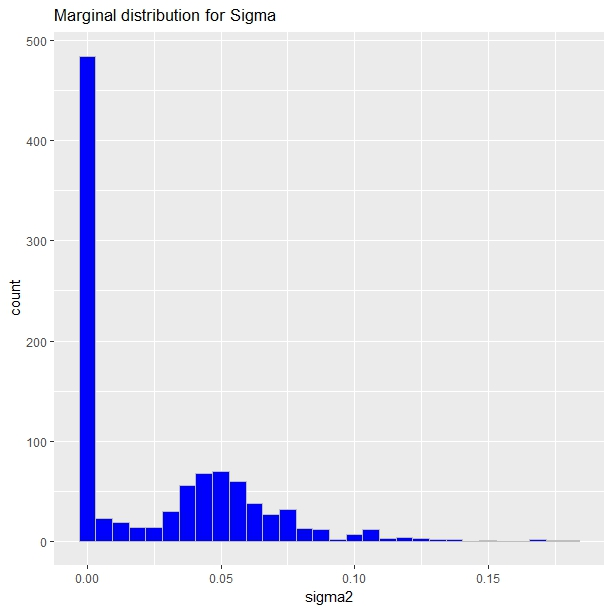
\includegraphics[width=.4\textwidth]{task5/CSMC_sigma2.jpeg}
	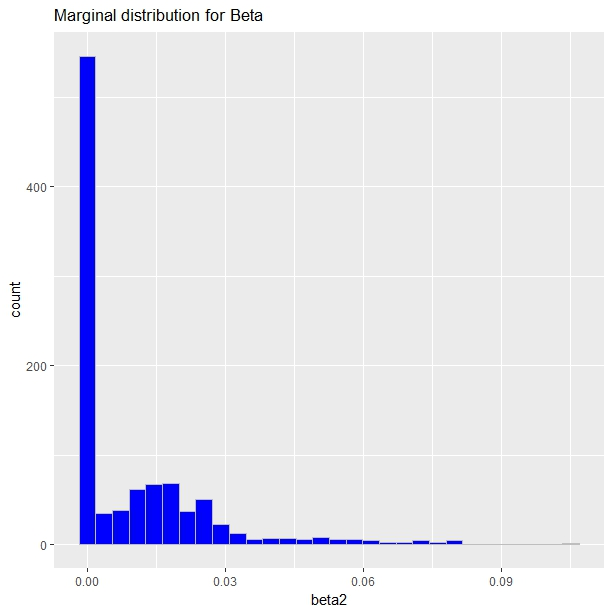
\includegraphics[width=.4\textwidth]{task5/CSMC_beta2.jpeg}
\end{center}

\subsection*{Question 15}
As we can notice from the plots, our implementation does not work properly, since the marginal distributions provided are not the same. 

Anyway, we provide the convergence rates for the two methods.

Using Gibbs sampler, we obtain a trace that suits the one of an $Inverse Gamma$ for $\sigma^2$, but the one of $\beta^2$ corresponds to a $Gaussian$, as we can see in the following plots.
\begin{center}
	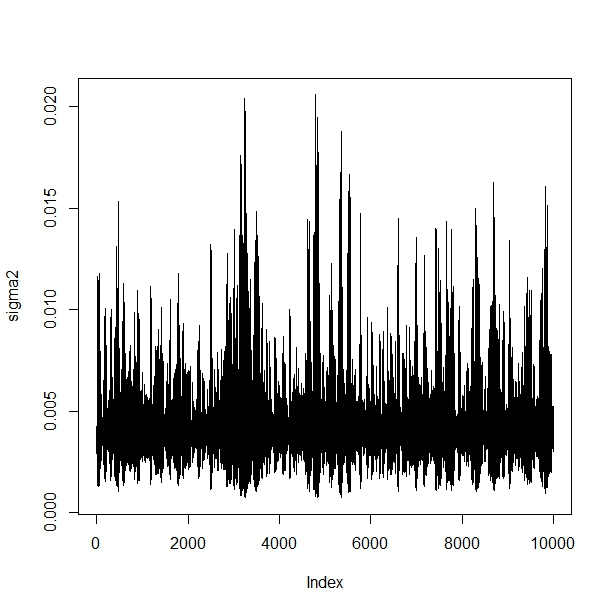
\includegraphics[width=.4\textwidth]{task5/Gibbs_sigma2_convergence.jpeg}
	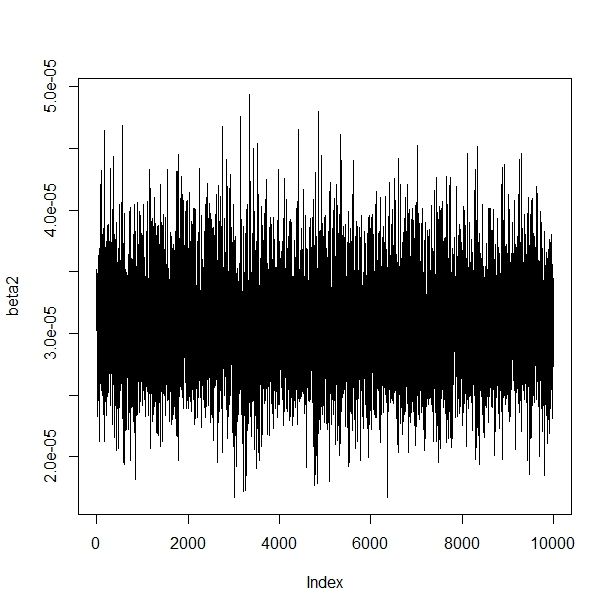
\includegraphics[width=.4\textwidth]{task5/Gibbs_beta2_convergence.jpeg}
\end{center}

Using CSMC, we obtain
\begin{center}
	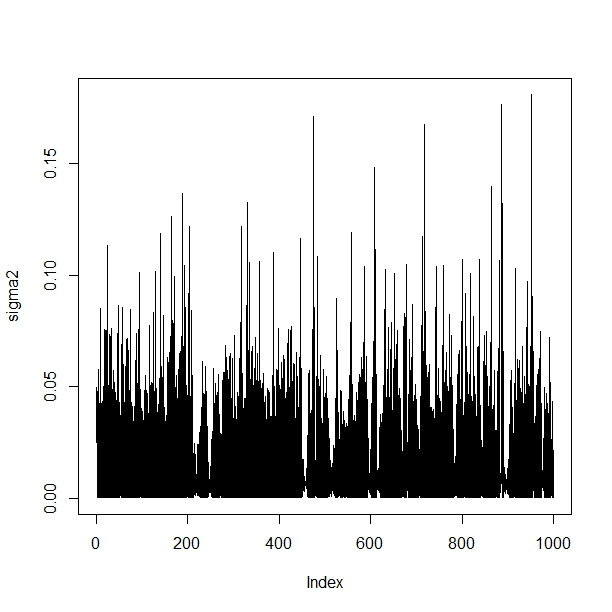
\includegraphics[width=.4\textwidth]{task5/CSMC_sigma2_convergence.jpeg}
	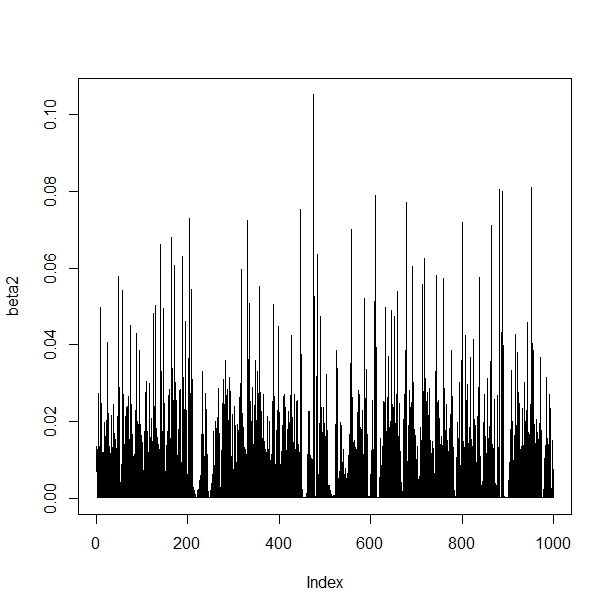
\includegraphics[width=.4\textwidth]{task5/CSMC_beta2_convergence.jpeg}
\end{center}

\newpage


\section*{3.2 Predicting a relation based on Indian Buffet Process}
Let us suppose that we observe the interactions between a set of entities and we wish to extract informative representations that are useful for making predictions about the entities and their relationships. One basic challenge is link prediction, where we observe the relationships (or “links”) between some pairs of entities in a network (or “graph”) and we try to predict unobserved links. 

In our model, each entity is described by a set of binary features. We are not given these features a priori and will attempt to infer them. We assume that the probability of having a link from one entity to another is entirely determined by the combined effect of all pairwise feature interactions. If there are $K$ features, then let $Z$ be the $N \times K$ binary matrix where each row corresponds to an entity and each column corresponds to a feature such that
$$ 
z_{ik} \equiv Z(i,k) = 
\begin{cases}
	1 \text{\ \ \ if the $i^{th}$ entity has feature $k$} \\
	0 \text{\ \ \ otherwise}
\end{cases}
$$
Let $Z_i$ denote the feature vector corresponding to entity $i$.

Let $W$ be a $K \times K$ real-valued weight matrix where $w_{kk'} \equiv W(k, k')$ is the weight that affects the probability of there being a link from entity $i$ to entity $j$ if both entity $i$ has feature $k$ and entity $j$ has feature $k'$.

Then the likelihood is defined as follows:
$$
Pr(y_{ij}=1|Z,W) = \prod_{i,j}Pr(y_{ij}|Z_i,Z_j,W)
$$
Given the feature matrix $Z$ and the weight matrix $W$, the probability that there is a link from entity $i$ to entity $j$ is
$$
Pr(y_{ij}=1|Z,W) = \sigma(Z_iWZ_j^T) = \sigma(\sum_{k,k'}z_{ik}z{jk'}w_{kk'}) 
$$
where $\sigma(\cdot)$ is a function that transforms values on $(-\infty, \infty)$ to $(0,1)$ such as the sigmoid function $\sigma(x) = (1+e^{-x})^{-1}$.

Given the full set of observations $X$, we wish to infer the posterior distribution of the feature matrix $Z$ and the weight $W$.

Without any prior knowledge about the features or their weights, a natural prior for $W$ is given by 
$$
w_{kl} \sim \mathcal{N}(0,\sigma^2).
$$

We generate the feature matrix $Z$ using the Indian Buffet Process. Each row of $Z$ corresponds to a diner at an Indian buffet; each column corresponds to a dish at the infinitely long buffet. If a customer takes a particular dish, then the entry that corresponds to the customer's row and the dish's column is a 1, otherwise the entry is 0. The first customer chooses a $Poisson(\alpha)$ number of dishes to sample; the $i^{th}$ customer tries each previously sampled dish with probability proportional to the number of people that have already tried the dish and then samples a $Poisson(\frac{\alpha}{i})$ number of new dishes. 

We do inference implementing a MCMC sampler. At each iteration, we have to:
\begin{enumerate}
	\item resample $Z$, given $W$;
	\item resample $W$, given $Z$.
\end{enumerate}

\subsection*{Question 19}
In the algorithm implementation that we provide, at first we create a binary feature matrix $Z$, using the Indian Buffet Process. As previously mentioned, The first customer chooses a $Poisson(\alpha)$ number of dishes to sample. Then, for each custumer $i$ we perform the following steps:
\begin{enumerate}
	\item [-] we compute the probability of visiting past dishes, given by $p = m_k/i$, where m is the number of customer that have already tried dish $k$;
	\item[-] sampling from a uniform distribution $\mathcal{U}(0,1)$, we either accept and set $z_{i,k}=1$ or reject the proposal;
	\item[-] we compute the number of new dishes visited by customer $i$, sampling from a $Poisson(\frac{\alpha}{i})$.
\end{enumerate}
Once $Z$ is built, we initialize the weight matrix $W$, using the fact that
$$
w_{kl} \sim \mathcal{N}(0,\sigma^2).
$$
Then, the MCMC sampler begins.
\begin{enumerate}
	\item To sample from the distribution defined by the IBP, we need to compute the conditional distribution $P(z_{ik}=1|Z_{-i,k})$, where $Z_{-i,k}$ denotes the entries of $Z$ other than $z_{ik}$. We have that
	$$
	P(z_{ik}=1|Z_{-i,k}) = \frac{m_{-i,k}+\frac{\alpha}{K}}{N+\frac{\alpha}{K}}
	$$
	where $m_{-i,k}$ is the number of customers that have tried dish $k$, not including $i$.
	
	So, for each column $k$ if $m_{-i,k}$  is greater than 0 we set $z_{ik}=1$ with probability given by the equation just stated. Otherwise, we delete that column. At the end of row $i$, we add $Poisson(\frac{\alpha}{N})$ new columns that have ones in that row. 
	\item We sequentially resample each of the weights in $W$ that correspond to non-zero features (or dishes) and drop all weights that correspond to all-zero features. 
	
	We use a Metropolis-Hastings step for each weight in which we propose a new weight from a Normal distribution centered around the old one. Then, the probability of accepting $w_{new}$, when the current weight is $w_{old}$ is given by
	\begin{align*}
		a(w_{new}|w_{old}) & = \frac{p*(w_{new})}{p*(w_{old})} \frac{q(w_{old}|w_{new})}{q(w_{new}|w_{old})} \\
		& = \frac{p(D|w_{new})p(w_{new})}{p(D|w_{old})p(w_{old})} \frac{q(w_{old}|w_{new})}{q(w_{new}|w_{old})} \\
		& = \frac{\sum_{i,j}\sigma(z_{ik}z_{jk}w_{kk',new})}{\sum_{i,j}\sigma(z_{ik}z_{jk}w_{kk',old})}\frac{p(w_{new})}{p(w_{old})}\frac{q(w_{old}|w_{new})}{q(w_{new}|w_{old})}
	\end{align*}
	knowing that the prior over the weights is a $Gaussian$ centered in 0, with standard deviation $\sigma$, and the proposal of $w_{new}$ from $w_{old}$ is  $Gaussian$ centered in $w_{old}$, with standard deviation $\sigma$.
 \end{enumerate}

\subsection*{Question 20}
Running the algorithm with inizial parameters $N = 10$, $\alpha = 10$, $\sigma=0.5$ we have the following results.
\\
\begin{center}
	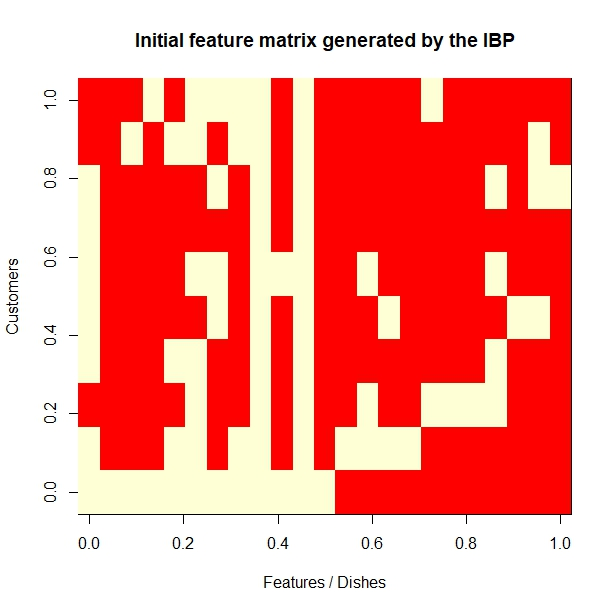
\includegraphics[width=8cm]{task7/output_initial_alpha10_sigma05_N10.jpeg}
\end{center}
As initial setting, $K=23$. After performing the MCMC sampler, we obtain
\\
\begin{center}
	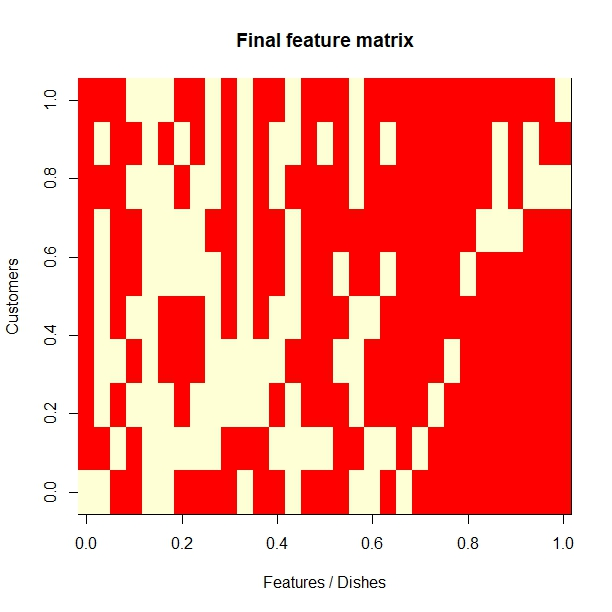
\includegraphics[width=9cm]{task7/output_final_alpha10_sigma05_N10.jpeg}
\end{center}
with $K=31$, using $10^3$ iterations for the sampling. 


\subsection*{Question 21}
Considering more customers, for instance $N=20$, our algorithm provides the following results.

As initial setting we have $K=37$. Initial and final feature matrices are:
\begin{center}
	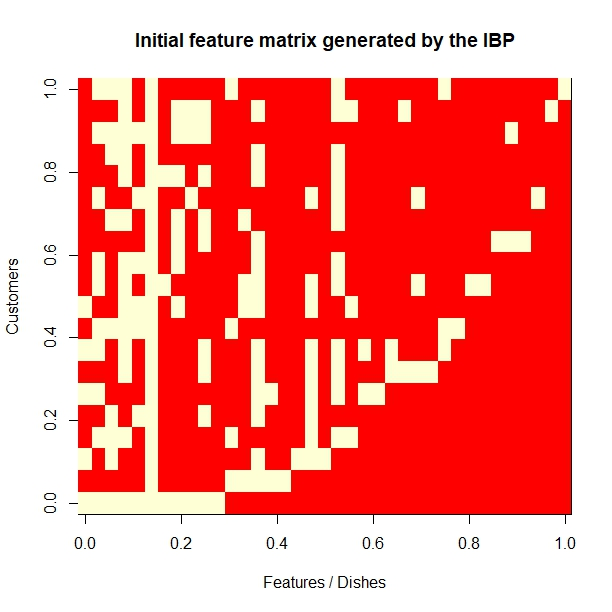
\includegraphics[width=.4\textwidth]{task7/output_initial_alpha10_sigma05_N20.jpeg}
	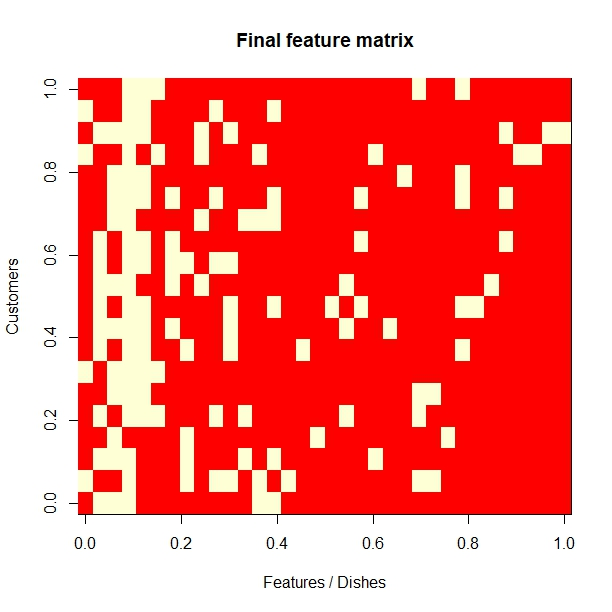
\includegraphics[width=.4\textwidth]{task7/output_final_alpha10_sigma05_N20.jpeg}
\end{center}
After the MCMC sampler we end up with $K=34$ features.

Varying the number of data points in the IBP slightly increases the number of clusters. This is because every extra data point (customer) gives the matrix another chance to add more features (dishes) from the distribution $Poisson(\frac{\alpha}{N})$.

Considering different values of $\alpha$, for instance $\alpha=5$, we have:
\begin{center}
	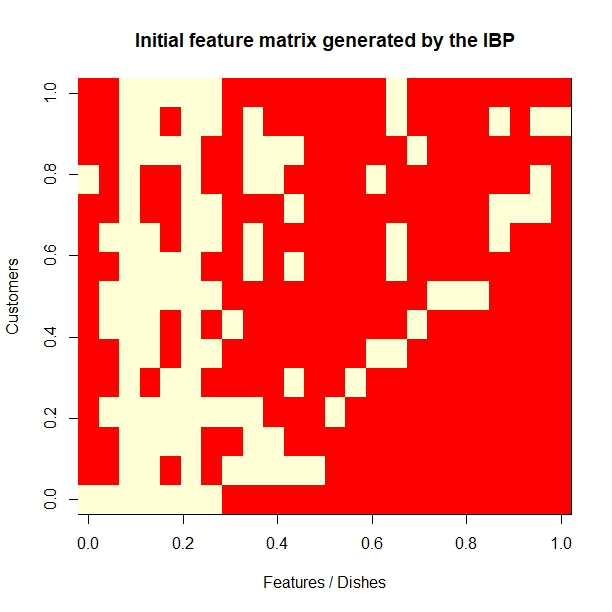
\includegraphics[width=.4\textwidth]{task7/output_initial_alpha5_sigma05_N15.jpeg}
	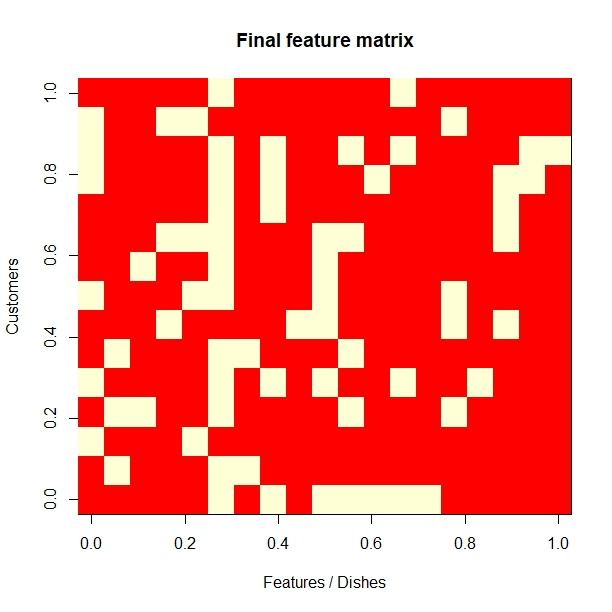
\includegraphics[width=.4\textwidth]{task7/output_final_alpha5_sigma05_N15.jpeg}
\end{center}
and we end up with $K=19$.

Setting $\alpha=15$, we have:
\begin{center}
	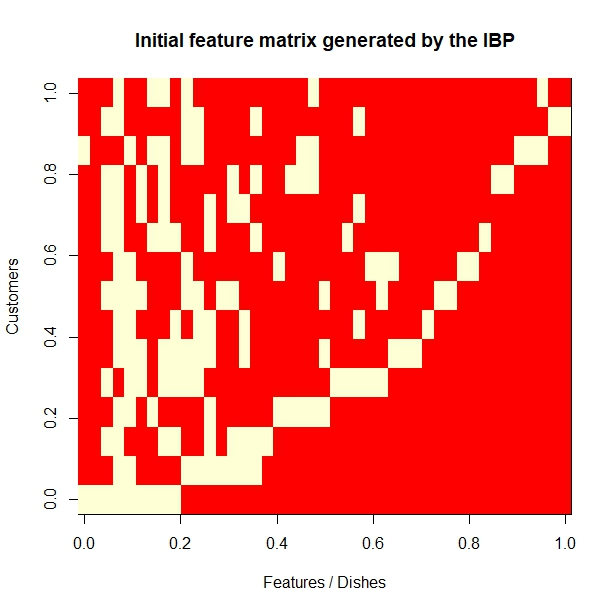
\includegraphics[width=.4\textwidth]{task7/output_initial_alpha15_sigma05_N15.jpeg}
	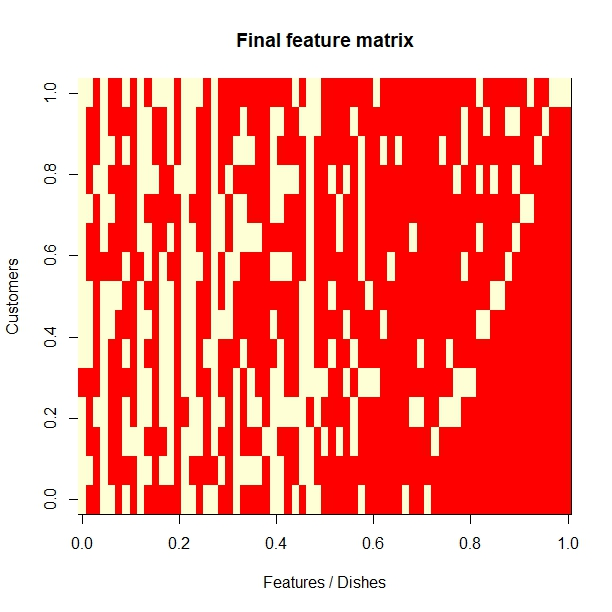
\includegraphics[width=.4\textwidth]{task7/output_final_alpha15_sigma05_N15.jpeg}
\end{center}
We started with $K=43$ and ended up with $K=67$ features.

We can conclude by saying that  $\alpha$ directly controls the total number of features and how readily features are added to the generated data. This is due to the fact that the number of new dishes added by the $i^{th}$ customer during the MCMC sampler is drawn directly from a $Poisson$ distribution parameterized by $\alpha$.

\end{document}

